% Chapter 3

\chapter{Chapter 3: Experiment} % Main chapter title

\label{Chapter 3} % For referencing the chapter elsewhere, use \ref{Chapter3} 

%----------------------------------------------------------------------------------------
\section{Experiment Intuition}
\label{sec:Experiment Intuition and Environment}
\paragraph{}
Existing experiments are generally simple both in state space and temporal structure, such as \citet{glascher2010states}, \citet{daw2011model}. They only examine the RL process in a two-stage decision making task. There is no evidence which RL algorithm will work when the problem becomes complicated. 

\paragraph{}
Besides, it seems that less is known about multi-task decision making. Previous work mostly use one reward function to see the learning process. But we do not know whether multiple-task simultaneous learning will cause tasks to assist or interfere with each other. 

\paragraph{}
Finally, the orders of tasks may further change the assistance or interference. 

\paragraph{}
With these questions, we defined our own experiment environment. 

\section{Experiment Environment}
\label{sec:Experiment Environment}
\subsection{Environment Structure}
\label{sec:Experiment Environment}
\paragraph{}
We create an abstract "labyrinth" environment for human to play. The labyrinth structure is displayed in Fig. \ref{fig:Environment Structure}. Each circle and the corresponding character represents a "state" participants may be in. The lines between states represents action's primary resulting states (we will explain the word "primary" in Section \ref{sec:Experiment Details}. Right now, you could just regard where the line points is its resulting state). It is obvious that the labyrinth consists of 6 states and each state has 3 actions, which point to 3 different resulting states. The goal for participants is to move from one state to another. For example, the participants may be asked to migrate from state \emph{A} to state \emph{B}. In this situation, the optimal solution is firstly move from \emph{A} to \emph{E}, and then go straight to \emph{B}. As a result, he successfully transmit himself from \emph{A} to \emph{B} in two steps. It is worth noting that participants know nothing about the structure of this environment before acting. Therefore, they could only know the structure by trying and learning. 

\begin{figure}[ht]
\centering
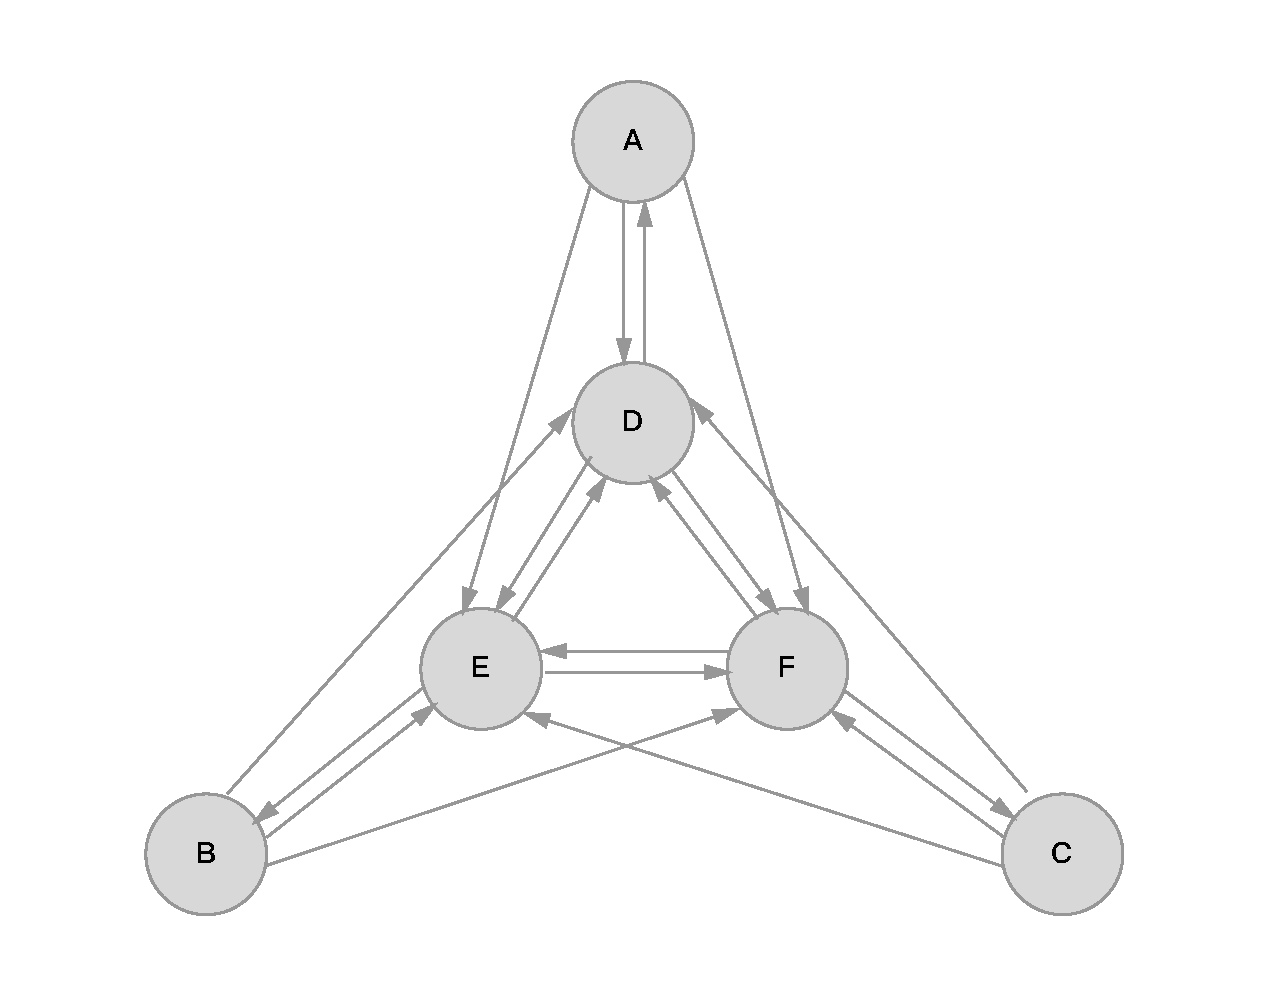
\includegraphics[width=\columnwidth]{Figures/environment_structure}
\decoRule
\caption[Environment Structure]{Environment Structure: circle indicates states (including \emph{A}, \emph{B}, \emph{C}, \emph{D}, \emph{E}, \emph{F}), line indicates action's primary consequence. }
\label{fig:Environment Structure}
\end{figure}

\paragraph{}
In this task, each states is represented by a fractal image, as shown in Fig. \ref{fig:fractal}. We chose 6 dissimilar fractal images to represent 6 different states. 

\begin{figure}[ht]
\centering
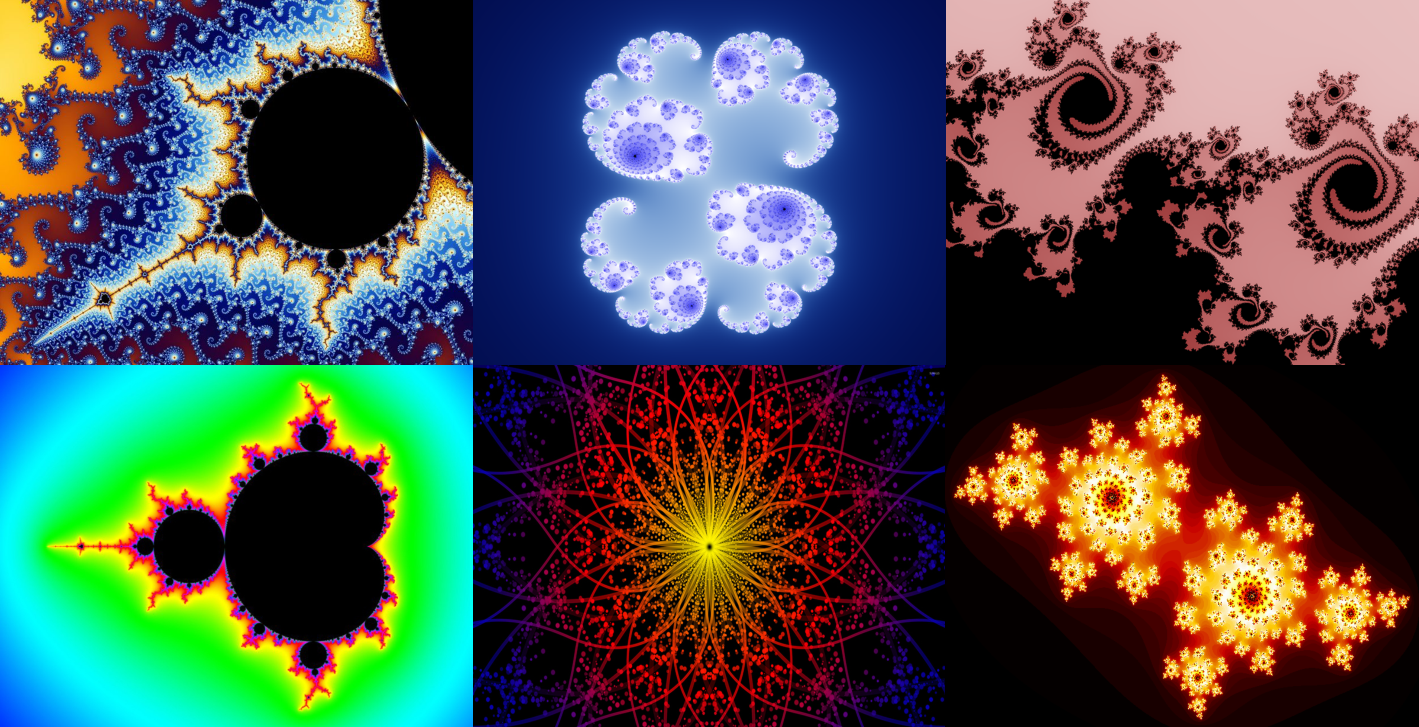
\includegraphics[width=\columnwidth]{Figures/fractal}
\decoRule
\caption{States Fractal Image}
\label{fig:fractal}
\end{figure}

\subsection{Trial Procedure}
\label{sec:Trial Procedure}
\paragraph{}
The Trial Procedure is demonstrated in Fig. \ref{fig:Experiment Procedure}. 
\paragraph{}
In the beginning of each trial, a fixation is displayed at the screen center for 1 second. After that, the trial start state and goal state are shown (start state at center, end state on the right) for 1.5 seconds. This is called preparation phase. Then, the free choice phase begins. 
\paragraph{}
At each timestep of free-choice phase, the state which the participant is now in is displayed in the center, being surrounded by three arrows indicating three kinds of actions. The goal state is always displayed on the right as in the preparation phase. Besides, there is a reward indication below the state, showing how much tokens participant could get if he reaches the end state after the next action. After the participant has made his decision and pressed one of three buttons, the center image will transit to the outcome state image with a fade-in fade-out fashion (previous image's $\alpha$ decreased gradually and new image's $\alpha$ increased gradually). In the meantime, reward indication will decrease by 1 (initially 20). But if the reward has been 1, it will not decrease but remain 1. There is no maximum reaction time, which means the screen will remain unchanged unless the participant press a button. When the transition ends, a new timestep begins. This is repeated until the state that participant is in reaches the end state. 
\paragraph{}
If participants have reached the end state, the trial enters feedback phase, in which total steps the participant takes to move to the end state and tokens earned are shown for 3 seconds. After feedback phase, a new trial begins with fixation. 

\begin{figure}[ht]
\centering
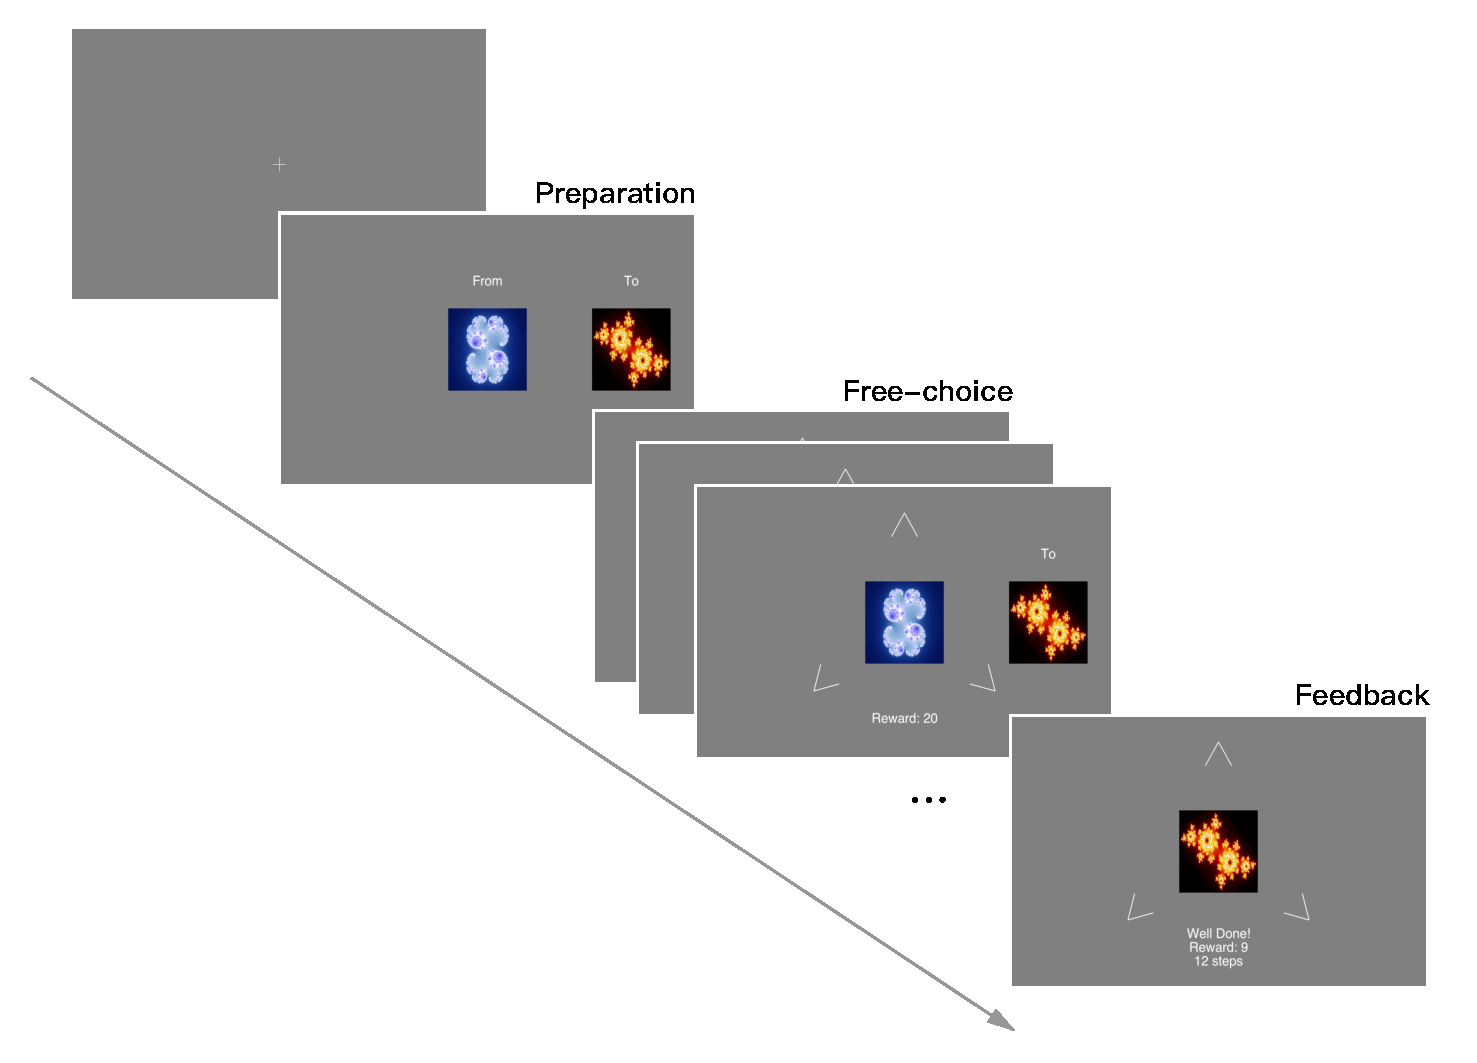
\includegraphics[width=\columnwidth]{Figures/experiment_procedure}
\decoRule
\caption{Experiment Procedure}
\label{fig:Experiment Procedure}
\end{figure}
%----------------------------------------------------------------------------------------


%----------------------------------------------------------------------------------------
\section{Experiment Design}
\label{sec:Experiment Design}
\paragraph{}
For every participant, there are totally 144 trials. each trial follows the procedure described in Section \ref{sec:Trial Procedure}. Till now, we haven't described how the start state and end state are chosen for each trial, and that's the key point of experiment design. 
\paragraph{}
The experiment is a between-subject design. The between-subject independent variable is the order of tasks and have two levels: randomized and block. Participants with odd participant id are assigned to block condition while participants with even participant id are assigned to randomized condition. For all conditions, whether randomized or block, the experiment consists of three kinds of start-end pairs: \emph{A} to \emph{B}, \emph{B} to \emph{C} and \emph{C} to \emph{A}. In short, the \enquote{inner} state \emph{D}, \emph{E}, \emph{F} will not be used as start or end state. The reason why we choose such tasks is that every task has an optimal solution of two steps. Just as the example shown in \ref{sec:Experiment Environment}, if the participant is asked to transit from \emph{A} to \emph{B}, he should take the path of \emph{A} -> \emph{E} -> \emph{B}, which takes two steps. You may also be wondering why we do not choose the opposite direction tasks, such as \emph{B} to \emph{A} as well. It is because we want to examine the possibility of knowledge transfer from previous tasks to newly occurred goals. For example, after learning how to move from \emph{A} to \emph{B} and from \emph{B} to \emph{C}, the participants are asked to do the task of \emph{C} to \emph{A}. In this manner, we want to test whether participants could transfer any knowledge from previous tasks, for instance, the structure of of environment, to the new tasks. That is exactly the difference between model-free and model-based algorithms. The overall trial number for each participant is 144. We divide 144 trials averagely into three tasks (\emph{A} to \emph{B}, \emph{B} to \emph{C} and \emph{C} to \emph{A}), making each one 44 trials. 
\paragraph{}
The experiment has 4 blocks, each of which contains 36 trials. 
For randomized condition, participants' tasks are assigned pseudo-randomly. For block condition, participants will only learn \emph{A} to \emph{B} in the first block, and then learn \emph{B} to \emph{C} in the second block, learn \emph{C} to \emph{A} in the third block. The final block of block condition consists of 12 trials for each task and the order is randomly assigned. In short, under randomized condition participants will learn all three tasks simultaneously while under block condition participants will learn the task one by one and finally test in the last block. 
%----------------------------------------------------------------------------------------


%----------------------------------------------------------------------------------------
\section{Experiment Details}
\label{sec:Experiment Details}
\paragraph{}
Now it is clear how the trial tasks are assigned and how a single trial proceeds. We still have several experiment details to explain. 
\paragraph{}
For the mapping from abstract state characters (such as \emph{A}) to fractal images, each participants received a randomly assigned mapping. In this case, the effect that specific images may cause can be balanced. 
\paragraph{}
For the mapping from state's action to \enquote{primary} consequence, it is also randomly assigned for each participant to avoid the possibility that specific optimal solution is preferred and relatively easy to learn for participants. 
\paragraph{}
The action's \enquote{primary} consequence mentioned in Section \ref{sec:Experiment Environment} means that in fact, action's consequence is stochastic in this environment. For a specific action of a state, it will have $0.7$ probability to transit to the primary consequence. However, it still have $0.2$ and $0.1$ probability to transit to other action's primary consequence of the same state. For example, the state \emph{A}'s first action's primary consequence is \emph{E}, while second action's primary consequence is \emph{D} and third action's primary consequence is \emph{F}. In this case, when participants chose the first action in state \emph{A}, it will transit to \emph{E} with probability $0.7$ and will transit to \emph{D} or \emph{F} with probability $0.2$ or $0.1$ (the one with $0.2$ probability is called \enquote{secondary} consequence, which is determined together with \enquote{primary} consequence when the environment is created). Thus, the action's consequence is stochastic actually. The reason why we add stochasticity here is to increase difficulty of the task, making it hard for participants to find the structure of our environment. As we mentioned in Section \ref{Chapter 1}, the existing work is mainly focused on laboratory toy problems, rather than real-world complex decision making. Though the complexity is still not comparable to real-world situations, it has been much more complex than previous tasks. 
\paragraph{}
The data our experiment records is the whole decision process, including every timestep's data of every trial. Each timestep data consists of current state, action chosen by participants, transition resulting state and reaction time. We will show how we analyze data in the following chapters. 
\paragraph{}
As for the reward, all the rewards participants collected in the experiment are tokens. The participant fee is calculated by $fee = 30 + tokens / 100$. An average participant may gain a fee of approximately 50 CNY. 
\paragraph{}
The data is collected on 36 Peking University students. They all have normal vision or corrected normal vision, including color vision. All participants had given informed consent before the experiment. 
%----------------------------------------------------------------------------------------




